

\tikzset{every picture/.style={line width=0.75pt}} %set default line width to 0.75pt        

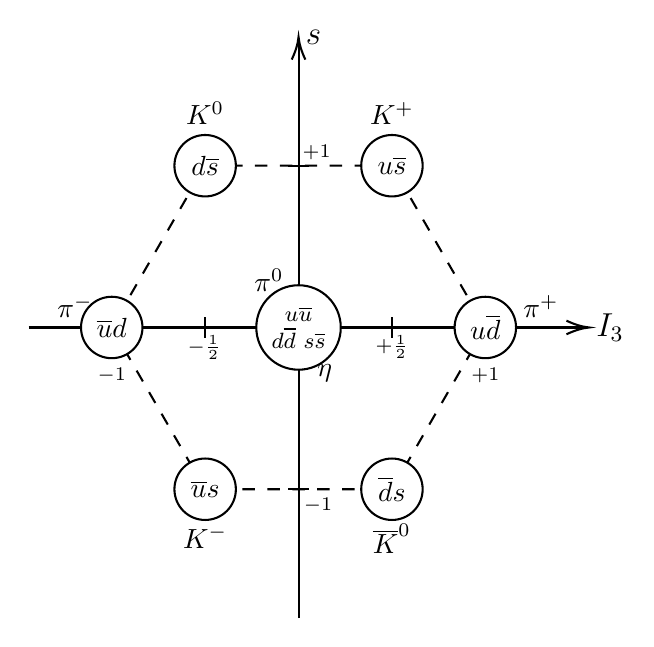
\begin{tikzpicture}[x=0.75pt,y=0.75pt,yscale=-1,xscale=1]
%uncomment if require: \path (0,470); %set diagram left start at 0, and has height of 470

%Shape: Regular Polygon [id:dp00036259320032794307] 
\draw  [dash pattern={on 4.5pt off 4.5pt}] (380,150) -- (335,227.94) -- (245,227.94) -- (200,150) -- (245,72.06) -- (335,72.06) -- cycle ;
%Straight Lines [id:da7432714490785992] 
\draw    (160,150) -- (428,150) ;
\draw [shift={(430,150)}, rotate = 180] [color={rgb, 255:red, 0; green, 0; blue, 0 }  ][line width=0.75]    (10.93,-3.29) .. controls (6.95,-1.4) and (3.31,-0.3) .. (0,0) .. controls (3.31,0.3) and (6.95,1.4) .. (10.93,3.29)   ;
%Straight Lines [id:da5800138783290809] 
\draw    (290,290) -- (290,12) ;
\draw [shift={(290,10)}, rotate = 90] [color={rgb, 255:red, 0; green, 0; blue, 0 }  ][line width=0.75]    (10.93,-3.29) .. controls (6.95,-1.4) and (3.31,-0.3) .. (0,0) .. controls (3.31,0.3) and (6.95,1.4) .. (10.93,3.29)   ;
%Straight Lines [id:da0424063895802933] 
\draw    (245,145) -- (245,155) ;
%Straight Lines [id:da5315540321645463] 
\draw    (335,145) -- (335,155) ;
%Shape: Circle [id:dp9016274878129079] 
\draw  [fill={rgb, 255:red, 255; green, 255; blue, 255 }  ,fill opacity=1 ] (230.2,72.06) .. controls (230.2,63.88) and (236.83,57.26) .. (245,57.26) .. controls (253.17,57.26) and (259.8,63.88) .. (259.8,72.06) .. controls (259.8,80.23) and (253.17,86.86) .. (245,86.86) .. controls (236.83,86.86) and (230.2,80.23) .. (230.2,72.06) -- cycle ;
%Shape: Circle [id:dp26967635701794923] 
\draw  [fill={rgb, 255:red, 255; green, 255; blue, 255 }  ,fill opacity=1 ] (320.2,72.06) .. controls (320.2,63.88) and (326.83,57.26) .. (335,57.26) .. controls (343.17,57.26) and (349.8,63.88) .. (349.8,72.06) .. controls (349.8,80.23) and (343.17,86.86) .. (335,86.86) .. controls (326.83,86.86) and (320.2,80.23) .. (320.2,72.06) -- cycle ;
%Shape: Circle [id:dp829825410707284] 
\draw  [fill={rgb, 255:red, 255; green, 255; blue, 255 }  ,fill opacity=1 ] (185.2,150) .. controls (185.2,141.83) and (191.83,135.2) .. (200,135.2) .. controls (208.17,135.2) and (214.8,141.83) .. (214.8,150) .. controls (214.8,158.17) and (208.17,164.8) .. (200,164.8) .. controls (191.83,164.8) and (185.2,158.17) .. (185.2,150) -- cycle ;
%Shape: Circle [id:dp7821465181120492] 
\draw  [fill={rgb, 255:red, 255; green, 255; blue, 255 }  ,fill opacity=1 ] (365.2,150) .. controls (365.2,141.83) and (371.83,135.2) .. (380,135.2) .. controls (388.17,135.2) and (394.8,141.83) .. (394.8,150) .. controls (394.8,158.17) and (388.17,164.8) .. (380,164.8) .. controls (371.83,164.8) and (365.2,158.17) .. (365.2,150) -- cycle ;
%Shape: Circle [id:dp050740490078981626] 
\draw  [fill={rgb, 255:red, 255; green, 255; blue, 255 }  ,fill opacity=1 ] (230.2,227.94) .. controls (230.2,219.77) and (236.83,213.14) .. (245,213.14) .. controls (253.17,213.14) and (259.8,219.77) .. (259.8,227.94) .. controls (259.8,236.12) and (253.17,242.74) .. (245,242.74) .. controls (236.83,242.74) and (230.2,236.12) .. (230.2,227.94) -- cycle ;
%Shape: Circle [id:dp8501124972426272] 
\draw  [fill={rgb, 255:red, 255; green, 255; blue, 255 }  ,fill opacity=1 ] (320.2,227.94) .. controls (320.2,219.77) and (326.83,213.14) .. (335,213.14) .. controls (343.17,213.14) and (349.8,219.77) .. (349.8,227.94) .. controls (349.8,236.12) and (343.17,242.74) .. (335,242.74) .. controls (326.83,242.74) and (320.2,236.12) .. (320.2,227.94) -- cycle ;
%Shape: Circle [id:dp12490437005601918] 
\draw  [fill={rgb, 255:red, 255; green, 255; blue, 255 }  ,fill opacity=1 ] (269.65,150) .. controls (269.65,138.76) and (278.76,129.65) .. (290,129.65) .. controls (301.24,129.65) and (310.35,138.76) .. (310.35,150) .. controls (310.35,161.24) and (301.24,170.35) .. (290,170.35) .. controls (278.76,170.35) and (269.65,161.24) .. (269.65,150) -- cycle ;
%Straight Lines [id:da10691295631235598] 
\draw    (285,72.06) -- (295,72.06) ;
%Straight Lines [id:da40035051048673465] 
\draw    (285,227.9) -- (295,227.9) ;

% Text Node
\draw (292,10) node [anchor=west] [inner sep=0.75pt]  [font=\large]  {$s$};
% Text Node
\draw (432,150) node [anchor=west] [inner sep=0.75pt]  [font=\large]  {$I_{3}$};
% Text Node
\draw (290.5,60.65) node [anchor=north west][inner sep=0.75pt]  [font=\fontsize{0.71em}{0.85em}\selectfont]  {$+1$};
% Text Node
\draw (291.08,230.57) node [anchor=north west][inner sep=0.75pt]  [font=\fontsize{0.71em}{0.85em}\selectfont]  {$-1$};
% Text Node
\draw (200,168.2) node [anchor=north] [inner sep=0.75pt]  [font=\fontsize{0.71em}{0.85em}\selectfont]  {$-1$};
% Text Node
\draw (380,168.2) node [anchor=north] [inner sep=0.75pt]  [font=\fontsize{0.71em}{0.85em}\selectfont]  {$+1$};
% Text Node
\draw (335.09,152.28) node [anchor=north] [inner sep=0.75pt]  [font=\fontsize{0.71em}{0.85em}\selectfont]  {$+\frac{1}{2}$};
% Text Node
\draw (244.65,152.6) node [anchor=north] [inner sep=0.75pt]  [font=\fontsize{0.71em}{0.85em}\selectfont]  {$-\frac{1}{2}$};
% Text Node
\draw (245,72.06) node    {$d\overline{s}$};
% Text Node
\draw (335,72.06) node    {$u\overline{s}$};
% Text Node
\draw (200,150) node    {$\overline{u} d$};
% Text Node
\draw (380,150) node    {$u\overline{d}$};
% Text Node
\draw (245,227.94) node    {$\overline{u} s$};
% Text Node
\draw (335,227.94) node    {$\overline{d} s$};
% Text Node
\draw (245,53.86) node [anchor=south] [inner sep=0.75pt]    {$K^{0}$};
% Text Node
\draw (335,53.86) node [anchor=south] [inner sep=0.75pt]    {$K^{+}$};
% Text Node
\draw (245,244.14) node [anchor=north] [inner sep=0.75pt]    {$K^{-}$};
% Text Node
\draw (335,243.14) node [anchor=north] [inner sep=0.75pt]    {$\overline{K}^{0}$};
% Text Node
\draw (192.38,146.82) node [anchor=south east] [inner sep=0.75pt]    {$\pi ^{-}$};
% Text Node
\draw (396.8,146.6) node [anchor=south west] [inner sep=0.75pt]    {$\pi ^{+}$};
% Text Node
\draw (284.27,134.09) node [anchor=south east] [inner sep=0.75pt]    {$\pi ^{0}$};
% Text Node
\draw (297.6,166.55) node [anchor=north west][inner sep=0.75pt]    {$\eta $};
% Text Node
\draw (290,150) node  [font=\fontsize{0.8em}{0.96em}\selectfont] [align=left] {\begin{minipage}[lt]{24.07pt}\setlength\topsep{0pt}
\begin{center}
$\displaystyle u\overline{u}$\\$\displaystyle d\overline{d}$ $\displaystyle s\overline{s}$
\end{center}

\end{minipage}};


\end{tikzpicture}

